\documentclass[UTF8,11pt,a4paper]{ctexart}

\usepackage[a4paper,top=2.2cm,bottom=2.2cm,left=2.5cm,right=2.5cm]{geometry}

\usepackage{amsmath,amssymb}
\usepackage{graphicx}
\usepackage{booktabs}
\usepackage{float}
\usepackage{subcaption}
\usepackage{array}
\usepackage{enumitem}
\usepackage{caption}
\usepackage{fancyhdr}
\usepackage{lastpage}
\usepackage{hyperref}

% 直接使用原项目中的图片目录
\graphicspath{{outputs/figures/}{../outputs/figures/}}

\hypersetup{
    colorlinks=true,
    linkcolor=black,
    urlcolor=black
}

\setlength{\parindent}{2em}
\setlength{\parskip}{0.15em}
\renewcommand{\arraystretch}{1.2}
\captionsetup{font=small}

\pagestyle{fancy}
\fancyhf{}
\fancyhead[L]{\small CLIP 在 CIFAR-10 上的对比实验}
\fancyhead[R]{\small 实验报告}
\fancyfoot[C]{\small \thepage/\pageref{LastPage}}
\renewcommand{\headrulewidth}{0.4pt}

\title{\textbf{CLIP Zero-Shot、Prompt Engineering 与 Linear Probe 在 CIFAR-10 上的对比实验}}
\author{}
\date{2026 年 8 月 26 日}

\begin{document}

\maketitle

\begin{abstract}
本实验主要比较 CLIP ViT-B/32 在 CIFAR-10 上的几种分类方式，包括直接使用类别名的 Zero-shot、Single Prompt、Prompt Ensemble，以及冻结 CLIP image encoder 后训练 Linear Probe。实验结果中，class-name Zero-shot 的准确率为 87.38\%，最佳单 Prompt 为 89.03\%，Prompt Ensemble 为 88.87\%，Linear Probe 最终达到 93.76\%。从结果来看，Prompt 的写法确实会影响 Zero-shot 分类，但提升幅度有限，而且不同类别对 Prompt 的敏感程度不一样。相比之下，Linear Probe 只训练一个很小的线性层就取得了更明显的提升，说明 CLIP 的视觉特征本身已经包含较强的类别判别信息。
\end{abstract}

\section{实验目的}

这次实验主要想回答下面几个问题：

\begin{enumerate}[leftmargin=2.3em]
    \item CLIP ViT-B/32 在 CIFAR-10 上直接做 Zero-shot 分类时的水平如何；
    \item 给类别名增加不同的自然语言模板后，准确率会发生多大变化；
    \item Prompt Ensemble 能否减少对特定 Prompt 写法的依赖；
    \item 若冻结 CLIP 的 image encoder，只训练一个线性分类器，效果和 Zero-shot 相比会怎么样；
    \item 哪些类别对 Prompt 比较敏感。
\end{enumerate}

\section{实验环境与数据}

\subsection{数据集}

实验使用 CIFAR-10 数据集。训练集包含 50,000 张图像，测试集包含 10,000 张图像，共 10 个类别：

\begin{center}
airplane、automobile、bird、cat、deer、dog、frog、horse、ship、truck。
\end{center}

所有图像都使用 CLIP 自带的 \texttt{preprocess} 进行预处理，没有再额外添加 normalization。

\subsection{模型}

所有实验都使用同一个 OpenAI CLIP ViT-B/32 checkpoint。图像特征和文本特征的维度都是 512。为了保证不同方法之间能够直接比较，实验过程中没有更换 backbone、checkpoint 和图像预处理方式。

\section{实验方法}

\subsection{Zero-shot Baseline}

最基础的设置是直接使用类别名作为文本输入。例如 airplane 类就只输入 ``airplane''，不添加其他描述。

对图像特征和文本特征分别进行 $L_2$ normalization，然后计算二者的 cosine similarity：

\begin{equation}
S = F_{\text{image}}F_{\text{text}}^{\top}.
\end{equation}

最后取相似度最大的类别作为预测结果。

\subsection{Single Prompt Engineering}

在类别名前后增加一个固定模板，测试了下面 4 个 Prompt：

\begin{itemize}
    \item \texttt{a photo of a \{\}}
    \item \texttt{a blurry photo of a \{\}}
    \item \texttt{a close-up photo of a \{\}}
    \item \texttt{an image of a \{\}}
\end{itemize}

\subsection{Prompt Ensemble}

Prompt Ensemble 对每个类别构造上面 4 个 Prompt。每个文本 embedding 先进行 $L_2$ normalization，再对 4 个 embedding 求平均，最后把平均后的向量再次 normalization：

\begin{equation}
\bar{t}_c =
\frac{
\frac{1}{K}\sum_{k=1}^{K}\hat{t}_{c,k}
}{
\left\|
\frac{1}{K}\sum_{k=1}^{K}\hat{t}_{c,k}
\right\|_2
},
\qquad K=4.
\end{equation}

这样做的目的不是为某一个类别单独挑最佳 Prompt，而是让结果不要过度依赖某一个固定写法。

\subsection{Linear Probe}

Linear Probe 中冻结 CLIP 的 image encoder，只使用提取出的 512 维归一化视觉特征训练一个线性分类器：

\begin{equation}
\text{Linear}: \mathbb{R}^{512}\rightarrow\mathbb{R}^{10}.
\end{equation}

线性层的参数量为 $512\times10+10=5,130$。

训练设置如表 \ref{tab:lp_setting} 所示。

\begin{table}[H]
\centering
\caption{Linear Probe 训练设置}
\label{tab:lp_setting}
\begin{tabular}{ll}
\toprule
参数 & 设置 \\
\midrule
Optimizer & AdamW \\
Learning rate & $1\times 10^{-3}$ \\
Weight decay & $1\times 10^{-4}$ \\
Epochs & 20 \\
Batch size & 256 \\
Trainable parameters & 5,130 \\
\bottomrule
\end{tabular}
\end{table}

\section{实验结果}

\subsection{Zero-shot Baseline}

只使用类别名时，测试集整体准确率为：87.38\%。

各类别准确率如表 \ref{tab:baseline_class} 所示。

\begin{table}[H]
	\centering
	\caption{Zero-shot class-name baseline 类别准确率}
	\label{tab:baseline_class}
	\setlength{\tabcolsep}{14pt}
	\renewcommand{\arraystretch}{1.15}
	\begin{tabular}{l c l c}
		\toprule
		类别 & 准确率 & 类别 & 准确率 \\
		\midrule
		airplane   & 81.30\% & dog   & 85.20\% \\
		automobile & 89.90\% & frog  & 77.00\% \\
		bird       & 91.70\% & horse & 97.10\% \\
		cat        & 79.20\% & ship  & 96.30\% \\
		deer       & 82.20\% & truck & 93.90\% \\
		\bottomrule
	\end{tabular}
\end{table}

可以看到，Zero-shot 的整体表现已经比较高，但是不同类别之间差异很明显。horse 和 ship 的准确率很高，而 frog、cat 和 airplane 相对较低。

\subsection{Single Prompt 结果}

不同 Prompt 的总体结果如表 \ref{tab:prompt_result} 所示。

\begin{table}[H]
\centering
\caption{Single Prompt Engineering 总体结果}
\label{tab:prompt_result}
\begin{tabular}{lrr}
\toprule
设置 & Accuracy & 相对 baseline \\
\midrule
class name & 87.38\% & -- \\
\texttt{a photo of a \{\}} & 88.83\% & +1.45 pp \\
\texttt{a blurry photo of a \{\}} & 87.86\% & +0.48 pp \\
\texttt{a close-up photo of a \{\}} & 86.93\% & $-$0.45 pp \\
\texttt{an image of a \{\}} & \textbf{89.03\%} & \textbf{+1.65 pp} \\
\bottomrule
\end{tabular}
\end{table}

最佳整体单模板是 \texttt{an image of a \{\}}。这个结果也说明 Prompt 并不是越长、越具体就越好。例如 \texttt{a close-up photo of a \{\}} 的准确率反而比只使用类别名低。

\subsection{Prompt Sensitivity}

这里把某个类别在全部 Prompt 设置中的最高准确率与最低准确率之差定义为 prompt sensitivity range。

实验中最敏感的类别是 frog，为 18.20 pp；最稳定的类别是 horse，为 1.60 pp。

两者差距比较大，说明 Prompt 对不同类别的影响确实不一样。

\subsection{Prompt Ensemble 结果}

Prompt Ensemble 的总体准确率为 88.87\%。

4 个成员 Prompt 的总体平均准确率是 88.16\%，标准差为 0.84 pp。Ensemble 相对成员平均提高了 0.71 pp，比最差成员高 1.94 pp，但仍然比最佳单 Prompt 低 0.16 pp。

从类别上看，Ensemble 在 9/10 个类别上超过了成员 Prompt 的平均表现。例如 frog 的 Ensemble 为 76.40\%，比成员均值高 2.33 pp，比最差 Prompt 高 13.80 pp。因此我认为 Ensemble 的主要作用更像是提高稳定性，而不是保证得到最高准确率。

\subsection{Linear Probe 结果}

Linear Probe 训练结束时得到：

\begin{itemize}
    \item Final train loss: 0.2288
    \item Final train accuracy: 93.55\%
    \item Training time: 7.93 s
\end{itemize}

在测试集上的准确率为 93.76\%。

它比 class-name Zero-shot 高 6.38 个百分点，比最佳单 Prompt 高 4.73 个百分点，比 Prompt Ensemble 高 4.89 个百分点。

\subsection{总体对比}

表 \ref{tab:overall} 汇总了四种主要方法的结果。

\begin{table}[H]
\centering
\caption{四种主要设置的总体结果}
\label{tab:overall}
\begin{tabular}{lrrl}
\toprule
设置 & Accuracy & 可训练参数 & Training Cost \\
\midrule
Zero-shot, class name & 87.38\% & 0 & 仅推理 \\
Best overall single prompt & 89.03\% & 0 & 仅推理 \\
Prompt Ensemble & 88.87\% & 0 & 仅推理 \\
Linear Probe & \textbf{93.76\%} & 5,130 & 7.93 s + 特征提取 \\
\bottomrule
\end{tabular}
\end{table}

\begin{figure}[H]
\centering
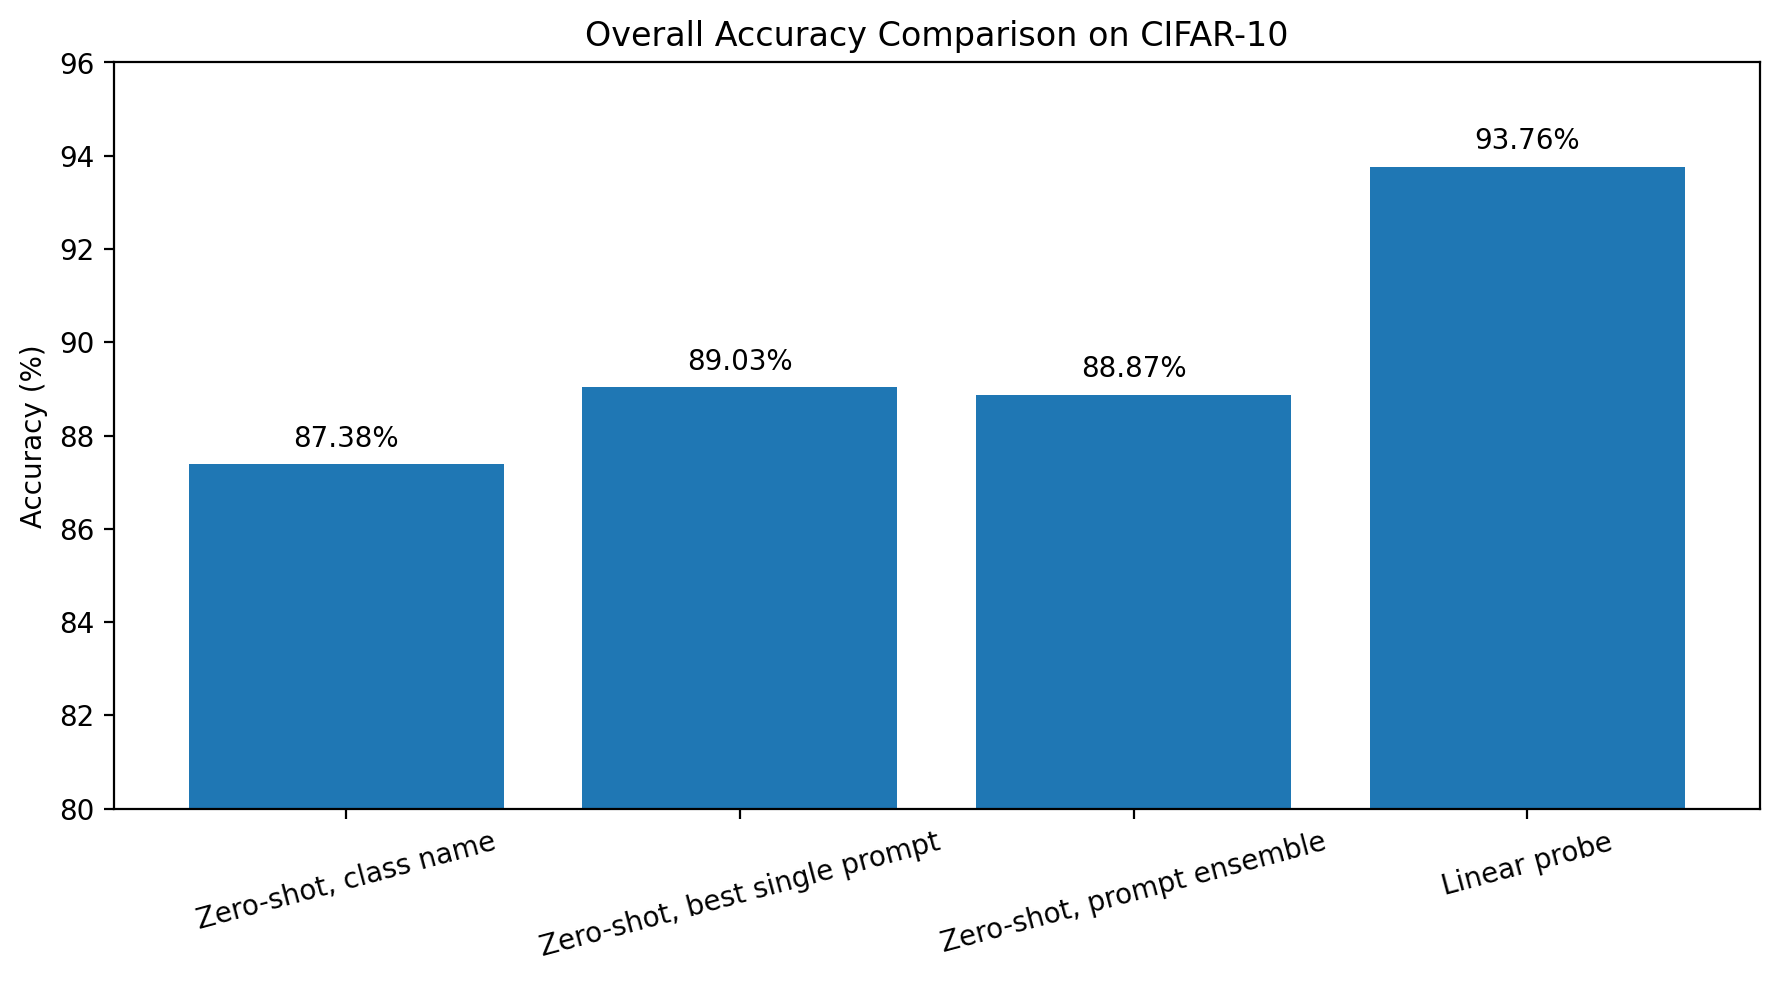
\includegraphics[width=0.78\textwidth]{overall_accuracy_comparison.png}
\caption{CIFAR-10 上四种方法的总体准确率比较}
\end{figure}

从总体结果看，Prompt Engineering 大概带来 1--2 个百分点以内的变化，而 Linear Probe 的提升更加明显。

\section{类别级结果分析}

不同方法的类别准确率如表 \ref{tab:class_all} 所示。

\begin{table}[H]
\centering
\small
\caption{不同方法的类别准确率（\%）}
\label{tab:class_all}
\begin{tabular}{lrrrr}
\toprule
Class & Zero-shot & Best overall prompt & Ensemble & Linear Probe \\
\midrule
airplane & 81.30 & 89.50 & 88.80 & 96.30 \\
automobile & 89.90 & 93.80 & 96.70 & 96.90 \\
bird & 91.70 & 87.50 & 88.10 & 89.80 \\
cat & 79.20 & 87.00 & 85.40 & 89.00 \\
deer & 82.20 & 78.90 & 79.60 & 91.90 \\
dog & 85.20 & 88.90 & 87.60 & 90.10 \\
frog & 77.00 & 75.40 & 76.40 & 95.40 \\
horse & 97.10 & 96.70 & 96.80 & 94.90 \\
ship & 96.30 & 95.70 & 96.70 & 96.40 \\
truck & 93.90 & 96.90 & 92.60 & 96.90 \\
\bottomrule
\end{tabular}
\end{table}

这里的 ``Best overall prompt'' 指总体准确率最高的统一模板 \texttt{an image of a \{\}}，不是对每个类别分别选择最佳 Prompt。

\begin{figure}[H]
\centering
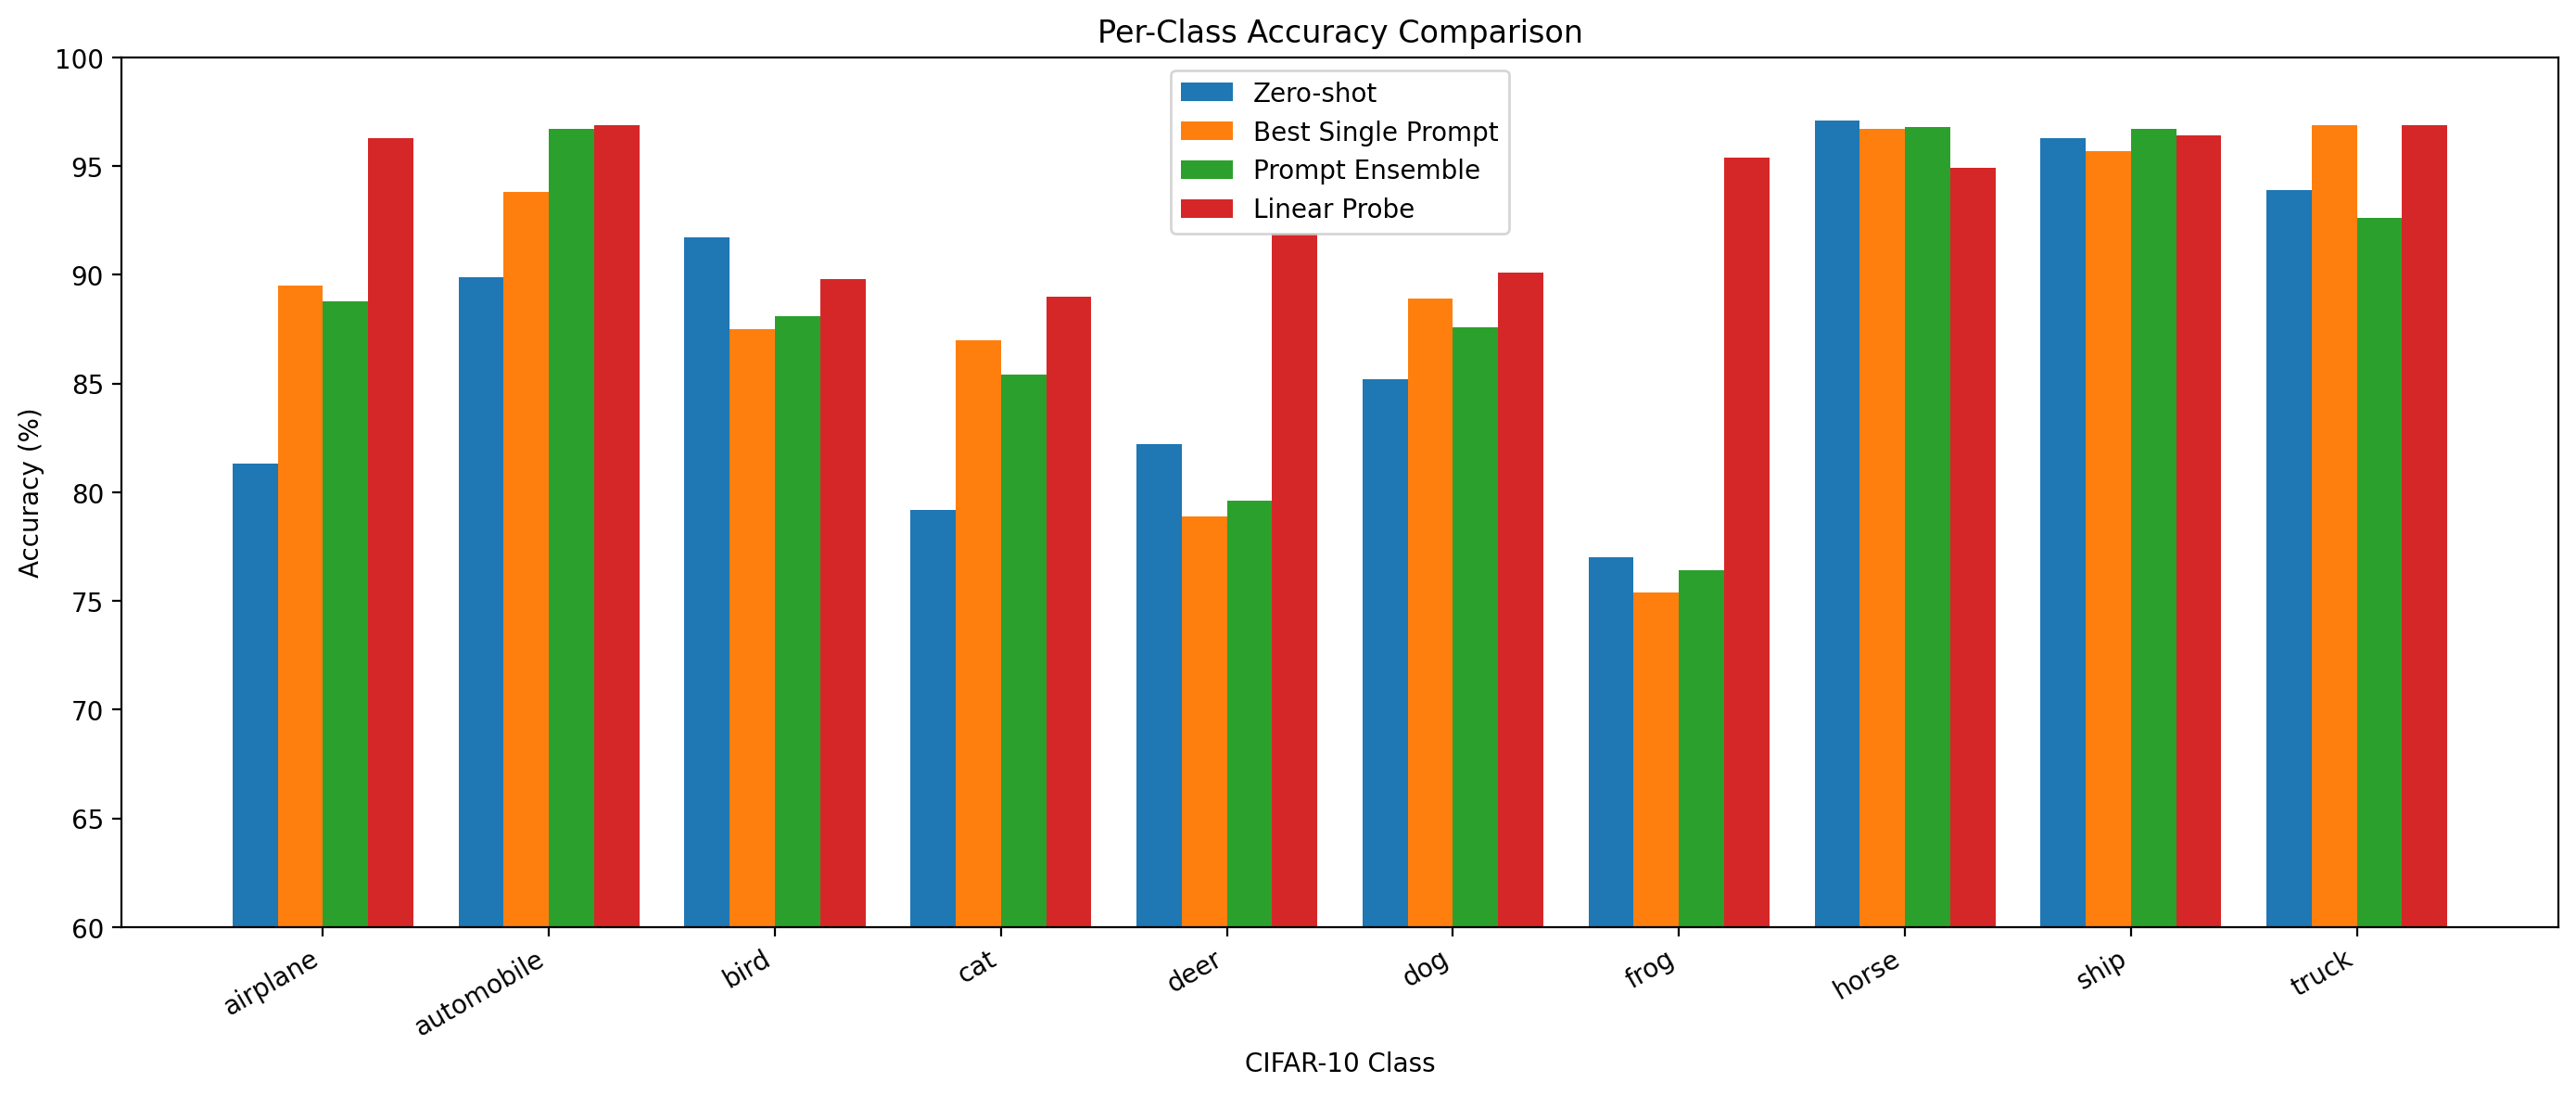
\includegraphics[width=0.95\textwidth]{per_class_accuracy_comparison.png}
\caption{不同方法的类别准确率比较}
\end{figure}

从 Zero-shot 到 Linear Probe，提升比较明显的类别有：

\begin{itemize}
    \item frog: +18.40 pp；
    \item airplane: +15.00 pp；
    \item cat: +9.80 pp；
    \item deer: +9.70 pp。
\end{itemize}

相反，horse 和 bird 分别下降 2.20 pp 和 1.90 pp。

我觉得 frog 是比较有代表性的类别。它一方面是 Prompt sensitivity 最大的类别，另一方面 Linear Probe 又能把准确率从 77.00\% 提升到 95.40\%。这说明 CLIP 的视觉特征中其实已经包含了较强的 frog 判别信息，Zero-shot 的限制更可能出现在文本类别表示与视觉特征的对齐方式上。

horse 的情况则相反。它在 class-name Zero-shot 下已经达到 97.10\%，Linear Probe 反而没有继续提高，说明这个类别和 CLIP 的文本语义空间本身就比较匹配。

\section{Confusion Matrix 分析}

Zero-shot 和 Linear Probe 的混淆矩阵如图 \ref{fig:cm} 所示。

\begin{figure}[H]
\centering
\begin{subfigure}{0.49\textwidth}
    \centering
    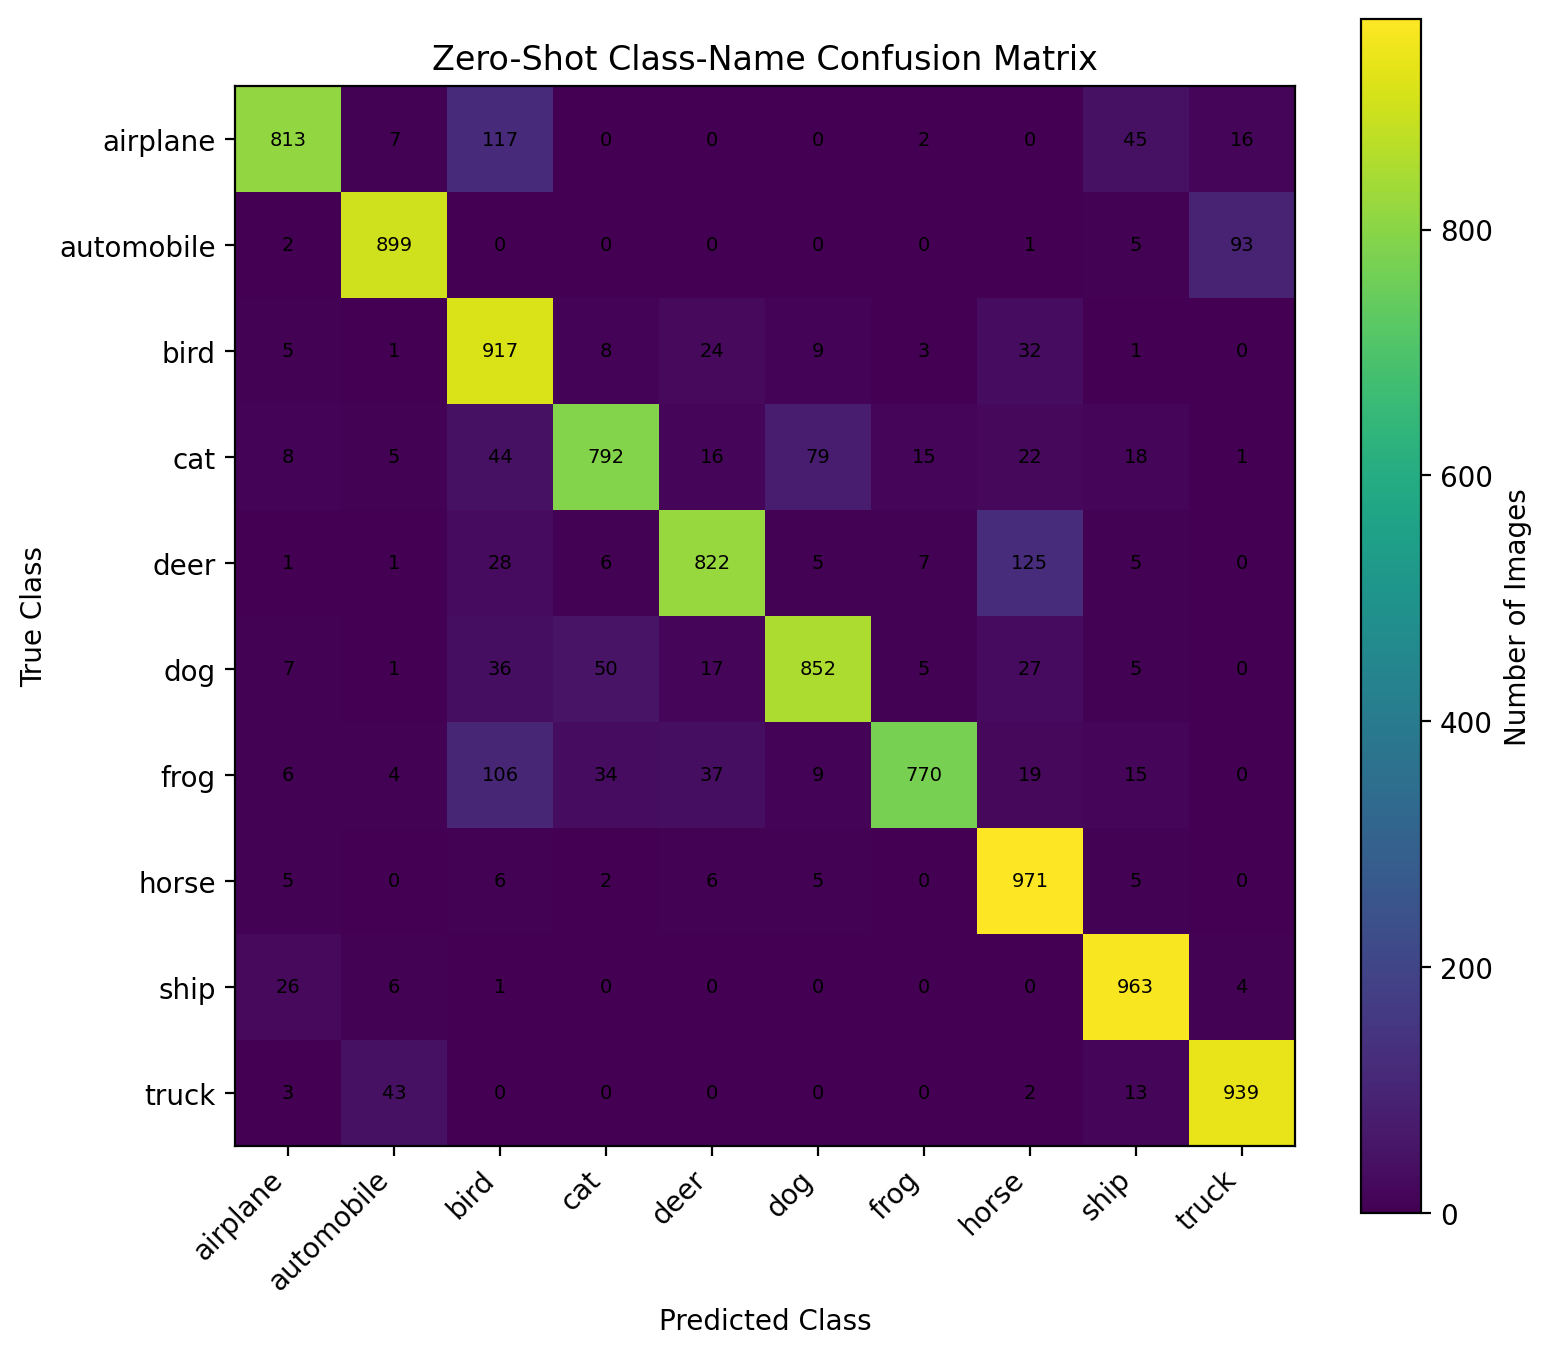
\includegraphics[width=\textwidth]{confusion_matrix_zero_shot.png}
    \caption{Zero-shot}
\end{subfigure}
\hfill
\begin{subfigure}{0.49\textwidth}
    \centering
    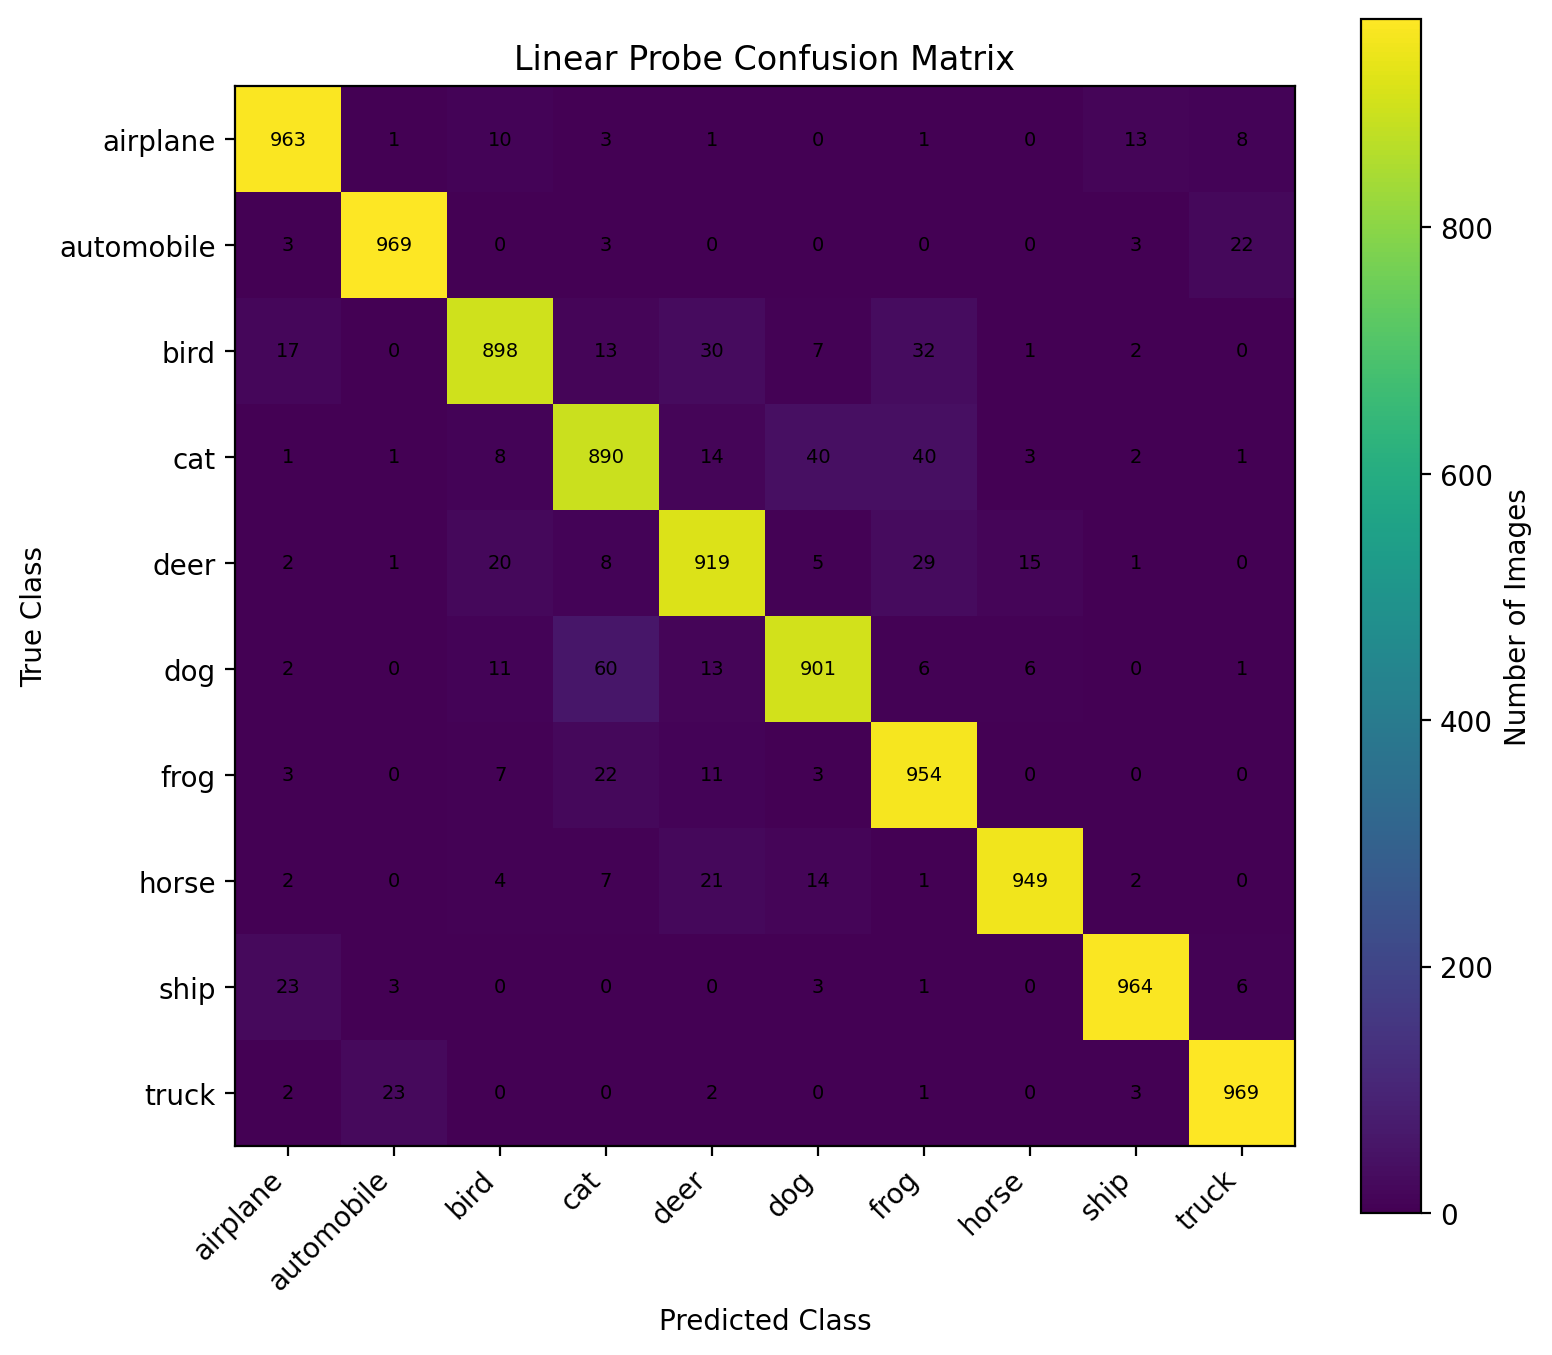
\includegraphics[width=\textwidth]{confusion_matrix_linear_probe.png}
    \caption{Linear Probe}
\end{subfigure}
\caption{Zero-shot 与 Linear Probe 的混淆矩阵}
\label{fig:cm}
\end{figure}

Zero-shot 中最大的单向混淆为 deer $\rightarrow$ horse: 125，Linear Probe 中最大的单向混淆为 dog $\rightarrow$ cat: 60。

从混淆矩阵可以看到，Linear Probe 确实减少了很多错误，但一些外观或语义比较接近的动物类别之间还是会出现混淆。

\section{结果讨论}

\subsection{Prompt Engineering 的作用}

从整体结果看，Prompt Engineering 是有效的，但增益没有特别大。最佳模板相对 baseline 提升了 1.65 pp，同时也存在模板使准确率下降的情况。

因此，Prompt Engineering 更像是在调整文本表示与视觉特征之间的匹配方式。它没有改变 image encoder，也没有真正增加新的视觉信息。

\subsection{Prompt Ensemble 的作用}

Prompt Ensemble 没有超过最佳单 Prompt，不过它比较接近最佳结果，并且比 4 个 Prompt 的平均表现更高。特别是在一些对 Prompt 比较敏感的类别上，它能明显减少最差 Prompt 带来的性能下降。

所以我认为 Ensemble 的意义主要是让结果更稳，而不是一定要把准确率做得更高。

\subsection{Linear Probe 说明了什么}

Linear Probe 只训练了 5,130 个参数，却能达到 93.76\%。这个结果说明 CLIP 的冻结视觉特征已经具有很强的线性可分性。

Zero-shot 和 Linear Probe 之间有 6.38 pp 的差距，这说明“视觉特征本身是否有信息”和“文本类别向量能不能把这些信息直接利用起来”并不是一回事。对于 frog、airplane、cat、deer 这类提升比较大的类别，Zero-shot 的瓶颈更可能是对齐问题，而不是 image encoder 完全没有学到相关视觉信息。

\section{结论}

通过这次实验，可以得到以下结论：

\begin{enumerate}[leftmargin=2.3em]
    \item CLIP ViT-B/32 在 CIFAR-10 上已经有较强的 Zero-shot 分类能力，只使用类别名就能达到 87.38\%；
    \item Prompt wording 会明显影响 Zero-shot 分类结果，而且不同类别的敏感程度不同；
    \item Prompt 写得更长、更具体不一定更好，部分 Prompt 甚至会让性能下降；
    \item Prompt Ensemble 的主要优势是降低对单个 Prompt 的依赖，让结果更加稳定；
    \item 冻结 CLIP image encoder 后，训练一个线性分类器可以达到 93.76\%，明显超过所有 Zero-shot Prompt 方法；
    \item Zero-shot 和 Linear Probe 的差距说明 CLIP 的视觉特征中包含了比当前文本 Prompt 能直接利用的更多类别判别信息。
\end{enumerate}

总体来说，这次实验让我比较直观地看到：Prompt Engineering 主要影响 CLIP 的图文对齐，而 Linear Probe 更能反映冻结视觉特征本身的分类能力。

\end{document}
